	\begin{center}
		\section{计数与组合}
	\end{center}

	\begin{multicols*}{2}

		\subsection{Catalan 数（合法括号串数量）}

		Catalan 数是一类专门计数“前缀不越界”结构的经典数列。第 $n$ 个 Catalan 数为：
		\[
			C_n = \frac{1}{n + 1}\binom{2n}{n}
			= \binom{2n}{n} - \binom{2n}{n + 1}.
		\]

		其中组合数相减的写法可以用反射法理解：先不管前缀限制，只要求 $n$ 个左括号和 $n$ 个右括号，总数是 $\binom{2n}{n}$。坏串是某个前缀中右括号第一次严格多于左括号的串。找到第一次使前缀和变为 $-1$ 的位置，把从开头到这个位置的括号全部翻转，例如 \texttt{())(()} 在第 $3$ 位第一次出错，翻转前三位得到 \texttt{)(((()}。这样坏串就会一一对应到含有 $n + 1$ 个左括号、$n - 1$ 个右括号的长度 $2n$ 串。反过来，对任意这样的串，找到第一次前缀和变为 $1$ 的位置并翻转前缀，就能还原唯一的坏串。因此坏串数量是 $\binom{2n}{n + 1}$，合法串数量即为 $\binom{2n}{n} - \binom{2n}{n + 1}$。

		最经典的含义是：长度为 $2n$ 的合法括号串数量。这里合法括号串要求恰好有 $n$ 个左括号和 $n$ 个右括号，并且任意前缀中左括号数量都不少于右括号数量。换成前缀和语言，就是把左括号看成 $+1$、右括号看成 $-1$，要求总和为 $0$ 且任意前缀和都不为负。

		例如 $n = 3$ 时，合法括号串共有 $C_3 = 5$ 个：
		\[
			\texttt{((()))},\quad
			\texttt{(()())},\quad
			\texttt{(())()},\quad
			\texttt{()(())},\quad
			\texttt{()()()}.
		\]

		竞赛中遇到类似模型时，不要只凭“像括号”就直接套 Catalan 数；先检查三个条件：对象能否编码成 $+1/-1$ 序列，最终总和是否固定，合法性是否只由前缀和下界决定。若终点为 $0$、下界为 $0$，就是标准 Catalan 数；若终点或下界发生偏移，通常要改用 Ballot 数或反射法的推广。合法括号串、栈的入栈/出栈过程、不过对角线的网格路径，都是同一个前缀约束的不同外壳。

		\subsection{求组合数（递推法）}

		会推这个杨辉三角吗？那你就会推组合数，一样的东西。

		\begin{minted}{cpp}
// c[a][b] 表示从a个苹果中选b个的方案数
for (int i = 0; i < N; i ++ )
		for (int j = 0; j <= i; j ++ )
	if (!j) c[i][j] = 1;
	else c[i][j] = (c[i - 1][j] + c[i - 1][j - 1]) % mod;
		\end{minted}

		\subsection{求组合数（逆元）}

		增加了这个如果传入参数有误（比如说顺序错了），输出报错信息的功能。

		\textcolor{red}{\textbf{Comb(x)初始化不能够传入 mod}}，最大传入 \verb|Comb(mod-1)|，传入 mod 会导致 \verb|frac[mod] = 0|，进而导致所有的 \verb|infrac| 变成 0。

		关于阶乘逆元的递推求法：由阶乘的定义可知：
		$$
		frac_{i+1} = frac_i \times (i+1)
		$$
		在模 $mod$ 意义下，等式两边同乘 $infrac_{i+1} \times infrac_i$ 进行化简，直接可得递推式：
		$$
		infrac_i \equiv infrac_{i+1} \times (i+1) \pmod{mod}
		$$
		因此，只需要用费马小定理先算出最大项 $n!$ 的逆元，便可 $O(n)$ 倒推算出所有的阶乘逆元。

		\begin{minted}{cpp}
namespace Comb{    // 组合数加逆元，依赖于这个MAXN（初始化）
	vector<ll> frac,infrac;
	int ln=1;
	bool initialized=false;
	// 在 k=0或者更小的时候 return 1
	inline ll binpow(ll a, ll k) {
		ll res = 1;
		a %= mod;
		while (k > 0) {
			if (k & 1) res = (res * a) % mod;
			a = (a * a) % mod;
			k >>= 1;
		}
		return res;
	}

	void Comb(int n) {
		ln = n;
		frac.assign(n + 5, 1);
		infrac.assign(n + 5, 1);
		for (int i = 1; i <= ln; ++i) {
			frac[i] = (frac[i - 1] * i) % mod;
		}
		infrac[ln] = binpow(frac[ln], mod - 2);
		for (int i = ln - 1; i >= 0; --i) {
			infrac[i] = (infrac[i + 1] * (i + 1)) % mod;
		}
	}

	inline ll CC(ll n, ll k) {
		if (k < 0 || k > n) {
#ifdef LOCAL
			cerr<<"CC 组合数传入参数不合法，可能是传入顺序错了\n";
#endif
			return 0; // Return 0 if k is out of range [0, n]
		}
		if(!initialized){
			Comb(MAXN);
			initialized=true;
		}
		ll res = frac[n];
		res = (res * infrac[n - k]) % mod;
		res = (res * infrac[k]) % mod;
		return res;
	}

	inline ll PP(ll n, ll k) {
		if (k < 0 || k > n) {
#ifdef LOCAL
			cerr<<"PP 排列数传入参数不合法，可能是传入顺序错了\n";
#endif
			return 0;
		}
		if(!initialized){
			Comb(MAXN);
			initialized=true;
		}
		ll res = frac[n] * infrac[n - k];
		res %= mod;
		return res;
	}
}
using namespace Comb;
		\end{minted}

		\subsection{插板法（stars and bars）求非负整数解的数量}
		\href{https://www.notion.so/stars-and-bars-3294539447bd8055a9e7fa3cac84be9e}{插板法（stars and bars）求非负整数解的数量} \\
		求解方程
		$$x_1 + x_2 + \cdots + x_n = A$$
		的解的个数（$A$ 为给定的正整数，$n$ 为变量个数）。

		\textbf{先看好理解的情形：$x_i \ge 1$。} 把和 $A$ 看成排成一行的 $A$ 个小球，相邻小球之间共有 $A - 1$ 个空隙。我们要把这一排球切成 $n$ 段，第 $i$ 段的球数就是 $x_i$。因为每段至少有一个球（对应 $x_i \ge 1$），所以只需在这 $A - 1$ 个空隙里插入 $n - 1$ 块隔板、每个空隙至多插一块即可。于是方案数就是从 $A - 1$ 个空隙里选 $n - 1$ 个的组合数：
		$$C_{A - 1}^{n - 1}$$
		这一步非常直观，所以插板法的“本体”其实就是 $x_i \ge 1$ 这个版本。

		\textbf{真正不好理解的是 $x_i \ge 0$。} 此时允许某一段为空，没法直接套“在空隙里插板”的图像。不过我们可以做一个代数变形，令
		$$y_i = x_i + 1 \quad (i = 1, 2, \cdots, n)$$
		由 $x_i \ge 0$ 立刻得到 $y_i \ge 1$；同时原方程两边各加上 $n$（共 $n$ 个 $+1$），右边变成 $A + n$：
		$$y_1 + y_2 + \cdots + y_n = A + n$$
		这样就把“$x_i \ge 0$、和为 $A$”的问题，\textcolor{blue}{\textbf{化归}}成了刚刚已经解决的“$y_i \ge 1$、和为 $A + n$”的问题。直接套用上面 $x_i \ge 1$ 的结论（把那里的 $A$ 换成 $A + n$）即得：
		$$C_{(A + n) - 1}^{n - 1} = C_{A + n - 1}^{n - 1} = C_{A + n - 1}^{A}$$

		\subsection{Lucas 定理}
		\href{https://www.notion.so/Lucas-3394539447bd804eaaeed232c7f86b4e}{Lucas 定理} \\
		注意，\textcolor{red}{\textbf{如果 $p$ 不是质数，那么 Lucas 定理不成立}}，而且这个 \textcolor{red}{\textbf{质数 $p$ 还是要求比较小的，一般就是 $10^6$ 以内。}}

		对于质数 $p$ 以及任意整数 $1 \le m \le n$，有如下同余式成立：
		$$C_{n}^{m} \equiv C_{n \bmod p}^{m \bmod p} \times C_{\lfloor n / p \rfloor}^{\lfloor m / p \rfloor} \pmod p$$

		代码实现如下：

		\begin{minted}{cpp}
// Lucas 定理递归求解，依赖于上方的组合数模板 CC 以及全局 mod
inline ll lucas(ll a, ll b) {
	// 如果 a, b 都小于 mod，直接通过预处理的 CC 求解组合数
	if (a < mod && b < mod) return CC(a, b);
	// 否则，根据 Lucas 定理递归求解
	return CC(a % mod, b % mod) * lucas(a / mod, b / mod) % mod;
}
		\end{minted}

		注意，在解决 Lucas定理 的时候，余数最大为 mod-1，所以只用预处理到 mod-1。\textcolor{red}{\textbf{绝对不能预处理到 mod}}，否则 \verb|frac[mod] = 0|，会导致所有的 \verb|infrac| 变成 0。

		\begin{minted}{cpp}
inline ll CC(ll n, ll k) {
	if (k < 0 || k > n) return 0;
	if(!initialized){
		// 【核心细节】：Lucas定理的余数最大为 mod-1，所以只用预处理到 mod-1。
		// 绝对不能预处理到 mod，否则 frac[mod] = 0，会导致所有的 infrac 变成 0。
		Comb(mod - 1);
		initialized = true;
	}
	ll res = frac[n];
	res = (res * infrac[n - k]) % mod;
	res = (res * infrac[k]) % mod;
	return res;
}
		\end{minted}

		\subsection{组合相关公式以及技巧}

		\subsubsection{离散变量概率变期望}

		当一个非负随机变量 $X$ 只取整数值时，其期望可以通过如下方式计算：
		$$E[X] = \sum_{i=1}^{\infty} P(X \ge i)$$
		即先对 $i = 1, 2, \dots$ 分别计算 $X \ge i$ 的概率，将这些概率相加即为期望。

		直觉上，期望的定义是 $E[X] = \sum_{k=1}^{\infty} k \cdot P(X=k)$，也就是每个取值 $k$ 贡献了 $k$ 份 $P(X=k)$。而 $P(X \ge i)$ 会把所有 $k \ge i$ 的概率加起来，所以 $\sum_{i=1}^{\infty} P(X \ge i)$ 中，取值 $k$ 恰好被 $i=1, 2, \dots, k$ 这 $k$ 个求和项各计入一次，合计贡献正好是 $k \cdot P(X=k)$，与期望定义吻合。

		这个技巧在概率题中非常常用：当直接求 $E[X]$ 困难时，转而对每个阈值 $i$ 求 $P(X \ge i)$ 往往更容易。

		\subsubsection{朱世杰恒等式（Hockey-stick identity）}

		$$C_i^i + C_{i+1}^i + \dots + C_n^i = C_{n+1}^{i+1}$$

		等价形式：
		$$\sum_{j=0}^{r} C_{i+j}^{i} = C_{i+r+1}^{i+1}$$

		\begin{center}
			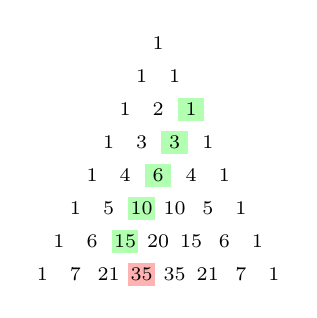
\begin{tikzpicture}[scale=0.42, every node/.style={font=\scriptsize}]
\def\rows{7}
\foreach \n in {0,...,\rows} {
	\foreach \k in {0,...,\n} {
		\pgfmathtruncatemacro{\val}{\n!/(\k!*(\n-\k)!)}
		\pgfmathsetmacro{\xpos}{-\n/2 + \k}
		\pgfmathsetmacro{\ypos}{-\n}
		\ifnum
			\n=2\ifnum
					\k=2
					\fill[green!30] (\xpos-0.4,\ypos-0.35) rectangle (\xpos+0.4,\ypos+0.35);
			\fi
		\fi
		\ifnum
			\n=3\ifnum
					\k=2
					\fill[green!30] (\xpos-0.4,\ypos-0.35) rectangle (\xpos+0.4,\ypos+0.35);
			\fi
		\fi
		\ifnum
			\n=4\ifnum
					\k=2
					\fill[green!30] (\xpos-0.4,\ypos-0.35) rectangle (\xpos+0.4,\ypos+0.35);
			\fi
		\fi
		\ifnum
			\n=5\ifnum
					\k=2
					\fill[green!30] (\xpos-0.4,\ypos-0.35) rectangle (\xpos+0.4,\ypos+0.35);
			\fi
		\fi
		\ifnum
			\n=6\ifnum
					\k=2
					\fill[green!30] (\xpos-0.4,\ypos-0.35) rectangle (\xpos+0.4,\ypos+0.35);
			\fi
		\fi
		\ifnum
			\n=7\ifnum
					\k=3
					\fill[red!30] (\xpos-0.4,\ypos-0.35) rectangle (\xpos+0.4,\ypos+0.35);
			\fi
		\fi
		\node at (\xpos,\ypos) {\val};
	}
}
			\end{tikzpicture}
		\end{center}

		杨辉三角，第 $0$ 行到第 $7$ 行。曲棍球棒恒等式确认，例如：对于 $n=6$，$r=2$：$1+3+6+10+15=35$。

		\textbf{应用}：当需要对连续上指标的组合数求和时（如 $\sum_{k=r}^{n}C_k^r$），可直接用朱世杰恒等式化为单个组合数 $C_{n+1}^{r+1}$，将 $O(n)$ 的求和降为 $O(1)$。

		\subsection{Hook-length 公式（树版本）：递增标号计数}

		有根树 $T$（$n$ 节点）上把 $1, \dots, n$ 填到节点、要求\textbf{每个非根节点标号 $>$ 父节点标号}（即整体是 min-heap / 递增树），合法方案数
		\[
			\#\{\text{递增标号}\} \;=\; \frac{n!}{\displaystyle\prod_{v \in T} \mathrm{size}(v)}.
		\]
		节点 $v$ 的「钩」就是它的整棵子树，钩长 $h(v) = \mathrm{size}(v) = |T_v|$。

		\textbf{直观概率法证明}。把 $1, \dots, n$ \textbf{均匀随机}分派到节点上（$n!$ 种等可能）。合法 min-heap $\Longleftrightarrow$ 每个 $v$ 是其子树 $T_v$ 的最小标号；单事件概率 $= 1/\mathrm{size}(v)$（$\mathrm{size}(v)$ 个位置地位对等）。这些事件\textbf{相互独立}——事件「$v$ 是 $T_v$ 最小」只看 $T_v$ 内部相对顺序，不同子树的相对顺序在均匀随机下互不影响。故合法概率 $\prod 1/\mathrm{size}(v)$，方案数 $= n! \cdot \prod 1/\mathrm{size}(v)$。$\blacksquare$

		\begin{center}
		\begin{forest}
			for tree={circle, draw, minimum size=1.7em, inner sep=0.5pt, s sep=6mm, l=8mm, edge={-}, font=\scriptsize},
			[$p_2$, fill=orange!30, label={[red, font=\tiny]right:$5$}
				[$p_1$, label={[red, font=\tiny]left:$1$}]
				[$p_4$, label={[red, font=\tiny]right:$3$}
					[$p_3$, label={[red, font=\tiny]left:$1$}]
					[$p_5$, label={[red, font=\tiny]right:$1$}]
				]
			]
		\end{forest}

		\vspace{2pt}
		{\footnotesize\sffamily\color{gray} 图注：$p = [3, 1, 4, 2, 5]$ 的笛卡尔树；\textcolor{orange!75!black}{橙} $=$ 根（全局最小）；\textcolor{red}{红字} $=$ 子树 $\mathrm{size}$。答案 $= 5!/(5 \cdot 1 \cdot 3 \cdot 1 \cdot 1) = 8$。}
		\end{center}

		\textbf{与笛卡尔树}。若能从 $a$ 唯一恢复 $\mathrm{prev}\_\mathrm{smaller} / \mathrm{next}\_\mathrm{smaller}$（即唯一定出笛卡尔树\textbf{形态}），则合法排列数 $= n! / \prod \mathrm{size}_i$，其中 $\mathrm{size}_i = \mathrm{left}_i + \mathrm{right}_i - 1$。\textbf{例题}：\href{https://codeforces.com/contest/2234/problem/E}{CF 2234E Vlad, Misha and Two Arrays}。

		\subsubsection*{拓展 1：杨表 Hook-length（原版，Frame--Robinson--Thrall 1954）}

		分拆 $\lambda = (\lambda_1 \ge \lambda_2 \ge \dots) \vdash n$ 对应 Young 图；标准杨表（SYT）是把 $1, \dots, n$ 填进 Young 图使得\textbf{每行严格递增、每列严格递增}。SYT 计数
		\[
			f^\lambda \;=\; \frac{n!}{\displaystyle\prod_{c \in \lambda} h(c)}, \qquad h(c) = \underbrace{r(c)}_{\text{同行右侧}} + \underbrace{d(c)}_{\text{同列下方}} + 1.
		\]

		本节的树版本就是这个公式在\textbf{树}上的类比（把 Young 图换成树、$h(c)$ 换成子树大小）。CP 里出现的场合：
		\begin{itemize}
			\item \textbf{$n$ 阶置换的 RSK 对应}：$n! = \sum_{\lambda \vdash n} (f^\lambda)^2$（每个 $\lambda$ 贡献 $(f^\lambda)^2$ 对 $(P, Q)$）。
			\item \textbf{长度 $\le k$ 的最长上升子序列}$= $ 第一行长度 $\le k$ 的杨表；配合 hook-length 可数计数。
			\item \textbf{格路计数}：从 $(0,0)$ 到 $(a, b)$、不越对角线的路径数 $= f^{(b, a)} / \text{显式化简} = $ Catalan / Ballot 数（Catalan 的另一种视角）。
		\end{itemize}

		\subsubsection*{拓展 2：森林 / 有序 vs 无序 / q-类}

		\begin{itemize}
			\item \textbf{森林版}：$n$ 节点森林（$k$ 棵根无序的树）的递增标号数 $= n! / \prod_v \mathrm{size}(v)$，跟单树公式一致（等价于加一个虚根统一）。
			\item \textbf{有序 vs 无序树}：本公式的树是「有孩子顺序」的（如笛卡尔树左右子树有别）。若树是无序的（同构算一次），除以每个节点的孩子置换群阶 $\prod_v |\mathrm{children}(v)|!$。
			\item \textbf{q-类版}：对树的\textbf{降序列}（descent）生成函数 $\sum_T q^{\mathrm{maj}(T)} = [n]_q! / \prod [\mathrm{size}(v)]_q$，其中 $[m]_q = (1 - q^m)/(1 - q)$。CP 少用但组合数学味浓，遇到"$q$-类比" / "$\mathrm{maj}$ 生成函数"题目时可想。
			\item \textbf{路径 / 链退化}：若树是一条链（$n$ 个节点从上到下），$\mathrm{size} = n, n-1, \dots, 1$，公式给 $n!/n! = 1$——链上只有唯一递增填法，符合直觉。
			\item \textbf{完全二叉树}：$n = 2^h - 1$ 层完全二叉树，$\prod \mathrm{size}$ 有闭式 $\prod_{k=0}^{h-1} (2^{h-k} - 1)^{2^k}$，可直接查表验证。
		\end{itemize}

		\subsection{Erd\H{o}s--Szekeres 定理（单调子序列）}

		任意 $n$ 个\textbf{互不相同}的实数构成的序列，只要长度
		\[
			n \ge (r - 1)(s - 1) + 1,
		\]
		就必含一个长度为 $r$ 的（严格）递增子序列，\textbf{或}一个长度为 $s$ 的（严格）递减子序列。

		取 $r = s = 3$：长度 $\ge (3 - 1)(3 - 1) + 1 = 5$ 的序列必含长度 $3$ 的单调子序列；反过来，\textcolor{blue}{\textbf{不含长度 $3$ 单调子序列的序列最长只有 $4$}}，临界长度恰好是 $5$。

		\textbf{鸽巢证明}：给每个位置记一对数 $(u, v)$——$u$ 是以它结尾的最长（非严格）递增子序列长度，$v$ 是最长递减长度。若全程不出现长度 $3$ 的单调子序列，则 $u, v \in \{1, 2\}$，组合只有 $2 \times 2 = 4$ 种；第 $5$ 个位置必与前面某位置的 $(u, v)$ 相同，而两位置标签相同会强制其中一维 $+1$，矛盾。故最长为 $4$。

		\begin{center}
		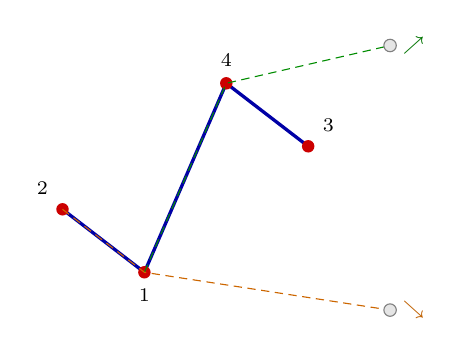
\begin{tikzpicture}[scale=0.8, font=\footnotesize,
			pt/.style={circle, fill=red!80!black, inner sep=0pt, minimum size=4.5pt},
			ghost/.style={circle, draw=gray, fill=gray!20, inner sep=0pt, minimum size=4.5pt}]
			% 锯齿 2 1 4 3：长度 4 的极大“无长 3 单调”序列
			\coordinate (p1) at (0, 2);
			\coordinate (p2) at (1.3, 1);
			\coordinate (p3) at (2.6, 4);
			\coordinate (p4) at (3.9, 3);
			\draw[very thick, blue!65!black] (p1) -- (p2) -- (p3) -- (p4);
			\node[pt, label={[font=\scriptsize]above left:$2$}] at (p1) {};
			\node[pt, label={[font=\scriptsize]below:$1$}]       at (p2) {};
			\node[pt, label={[font=\scriptsize]above:$4$}]       at (p3) {};
			\node[pt, label={[font=\scriptsize]above right:$3$}] at (p4) {};
			% 第 5 个点：放高 / 放低都崩
			\coordinate (hi) at (5.2, 4.6);
			\coordinate (lo) at (5.2, 0.4);
			\draw[densely dashed, green!55!black]  (p2) -- (p3) -- (hi);
			\draw[densely dashed, orange!80!black] (p1) -- (p2) -- (lo);
			\node[ghost] at (hi) {};
			\node[ghost] at (lo) {};
			\node[green!45!black,  right=1pt, font=\scriptsize] at (hi) {$\nearrow$};
			\node[orange!75!black, right=1pt, font=\scriptsize] at (lo) {$\searrow$};
		\end{tikzpicture}

		\vspace{2pt}
		{\footnotesize\sffamily\color{gray} 图注：\textcolor{blue!65!black}{蓝} $=$ 锯齿序列 $2\,1\,4\,3$（长度 $4$，任取 $3$ 个都不构成非严格单调，合法）；补第 $5$ 个点（灰）无论放高放低，都与前两点凑出长度 $3$ 单调子序列（\textcolor{green!45!black}{绿} $1 \le 4 \le 4.6$ 递增 / \textcolor{orange!75!black}{橙} $2 \ge 1 \ge 0.4$ 递减），故临界长度为 $5$。}
		\end{center}

		\textbf{应用}：统计「不含长度 $3$ 非严格单调子序列」的连续子段个数时，由本定理合法子段长度 $\le 4$，对每个右端点向左只需枚举长度 $1 \sim 4$ 暴力判定，$O(n)$ 完成。例题：\href{https://ac.nowcoder.com/acm/contest/113664/M}{牛客 河南萌新联赛 2025（一）M 无聊的子序列}（$n \le 10^6$）。该题是\textbf{非严格}版（允许相等），合法子段长度同样 $\le 4$；定理原版针对严格单调（元素互异），可与 Dilworth 定理、最长上升子序列对照理解。


	\end{multicols*}




